\chapter{MCSA Estimator and Fixed Point\\ Iteration Analysis\ }
\label{chap:spn_estimator_comparison}
The iterative performance of MCSA is studied in this appendix with
both the collision and expected value estimators using the ILUT
preconditioning. Although the expected value estimator achieved the
best iterative performance in analysis for the simple Poisson problem
in \S~\ref{sec:parameter_estimator_analysis}, it is possible that the
collision estimator may perform better from a timing perspective for
the $SP_N$ equations. The deterministic component of the expected
value estimator that couples the current state to other local states
through the iteration matrix stencil requires application of the
estimator to potentially several orders of magnitude more states at
every transition event.

For this study, the fuel assembly problem with a 1-group $SP_1$
discretization was solved using MCSA with the adjoint Monte Carlo
solver using both the collision and expected value estimators and both
the Richardson and minimal residual fixed point iterations. Using the
analysis from Appendix~\ref{chap:spn_mcsa_relaxation}, a Neumann
relaxation parameter of 0.7 was used with both estimators and fixed
point iterations. For the collision estimator, a Richardson relaxation
parameter of 1.1 was used with the Richardson iteration while it was
found the expected value estimator had the best performance when a
Richardson relaxation parameter of 1.0 was used instead. In addition,
ILUT preconditioning with a drop tolerance of \sn{1}{-5} and a fill
level of 5 was used with a reduced domain approximation fill level of
100 and a threshold of \sn{1}{-10} as in the previous
analysis. Artificial absorption was also introduced with a value of
0.2 for the MCSA calculations that used the collision estimator as CPU
timing performance was improved without a loss in iterative
performance while no absorption was used for calculations using the
expected value estimator. For each estimator, the number of stochastic
histories used to compute the MCSA correction was varied from 25 to
50,000 with the number of MCSA iterations required to converge to a
tolerance of \sn{1}{-8} recorded for a single eigenvalue iteration
along with the CPU time required to achieve convergence.

Figure~\ref{fig:spn_estimator_iters} gives the iteration count results
and Figure~\ref{fig:spn_estimator_time} gives the timing
results. Remarkably, although the fuel assembly problem is
significantly more complicated than the simple Poisson problem studied
in \S~\ref{sec:parameter_estimator_analysis}, the results here are
largely the same with Figure~\ref{fig:spn_estimator_iters} and
Figure~\ref{fig:estimator_nh_iters} having identical qualitative
behavior. Using the expected value estimator with both fixed point
iterations again creates a relative insensitivity to the number of
histories used to compute the correction. Marginally better iterative
and timing performance was observed for the expected value estimator
when using the Richardson iteration. Better timing performance is
expected as computing the extrapolation parameter in the minimal
residual iteration requires several additional parallel
operations. 

Compared to the collision estimator, the minimal residual iteration
permits fewer stochastic histories to be used with each MCSA iteration
while still maintaining good iterative performance. With respect to
CPU time, there is a more pronounced effect due to the larger density
of states created by the explicit ILUT preconditioning. Using a
reduced domain fill level of 100 creates a situation where the
expected value estimator is significantly more expensive per history
to compute that the collision estimator due to the coupling of states.
For the collision estimator, using around 20,000 stochastic histories
at every iteration gave the best iterative performance while 500
histories per iteration gave the best iterative performance when using
the expected value estimator. For purely serial computational
performance, there is not a distinguishing feature for the fuel
assembly problem presented that would cause one to choose one of the
estimators and fixed point iterations over the other.

\begin{figure}[t!]
  \begin{center}
    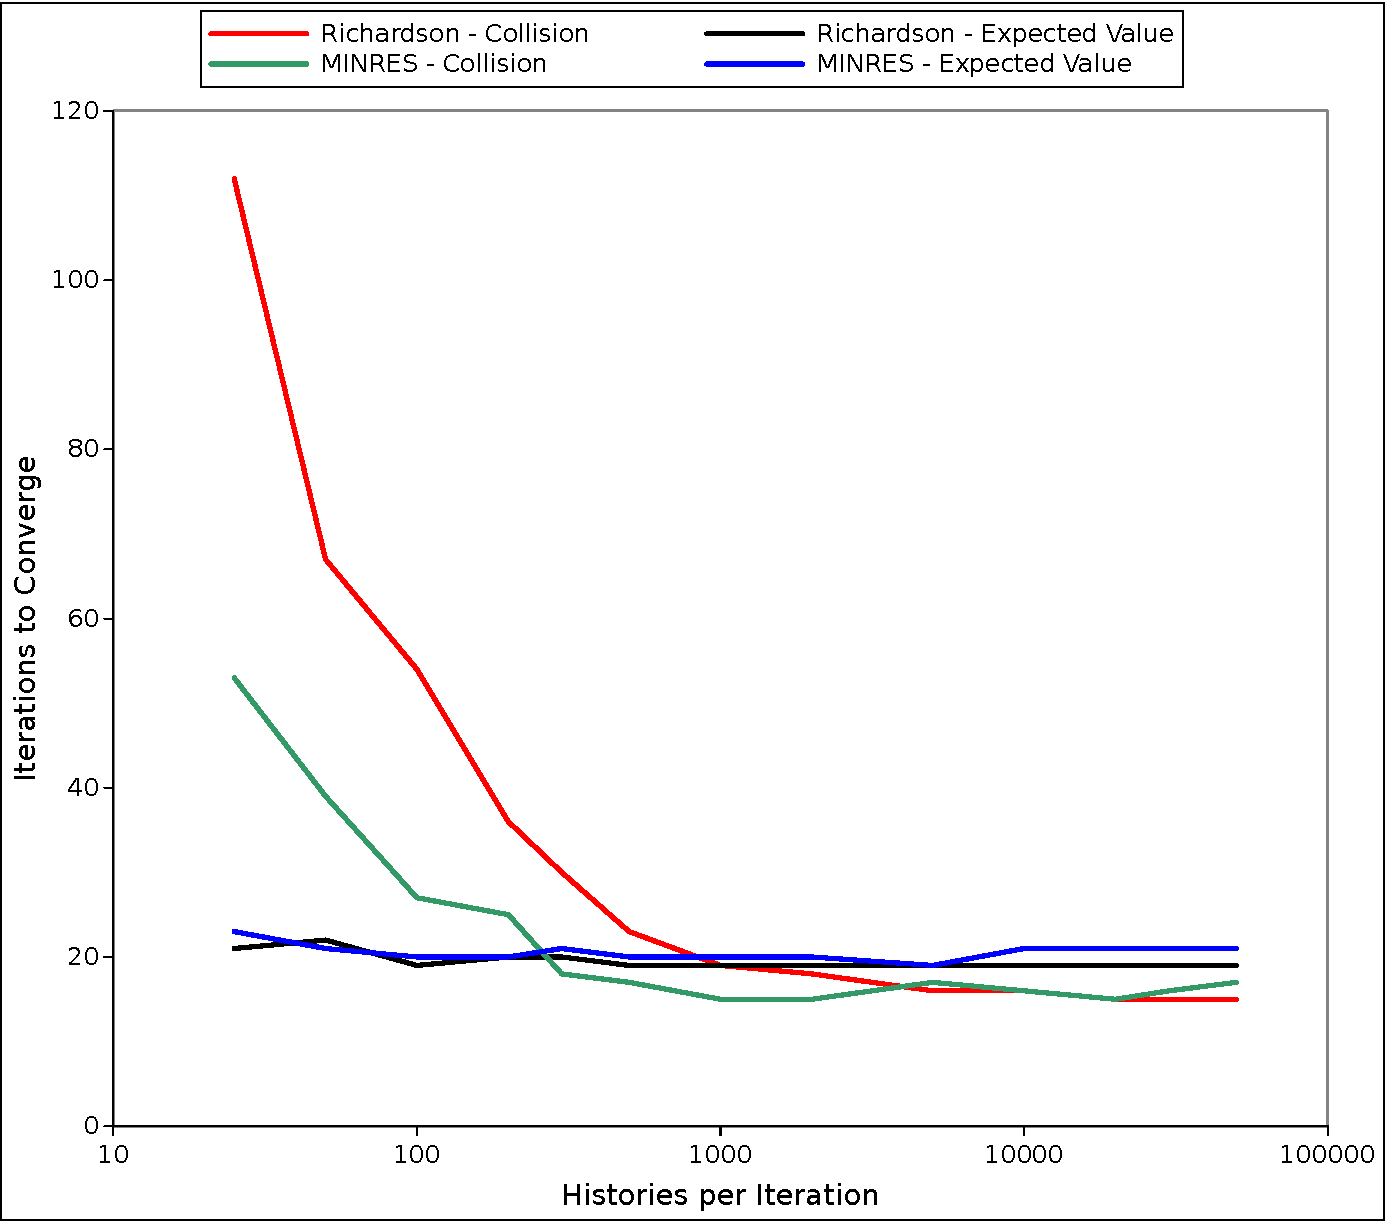
\includegraphics[width=5in]{chapters/spn_equations/estimator_iters.pdf}
  \end{center}
  \caption{\textbf{MCSA iterations required to converge the fuel
      assembly problem to a tolerance of \sn{1}{-8}.} \textit{Both the
      collision and expected value estimators were used with the
      adjoint Monte Carlo solver to compute the correction at each
      iteration. Each estimator was used with the Richardson and
      minimal residual fixed point iterations within an MCSA
      iteration.}}
  \label{fig:spn_estimator_iters}
\end{figure}

\begin{figure}[t!]
  \begin{center}
    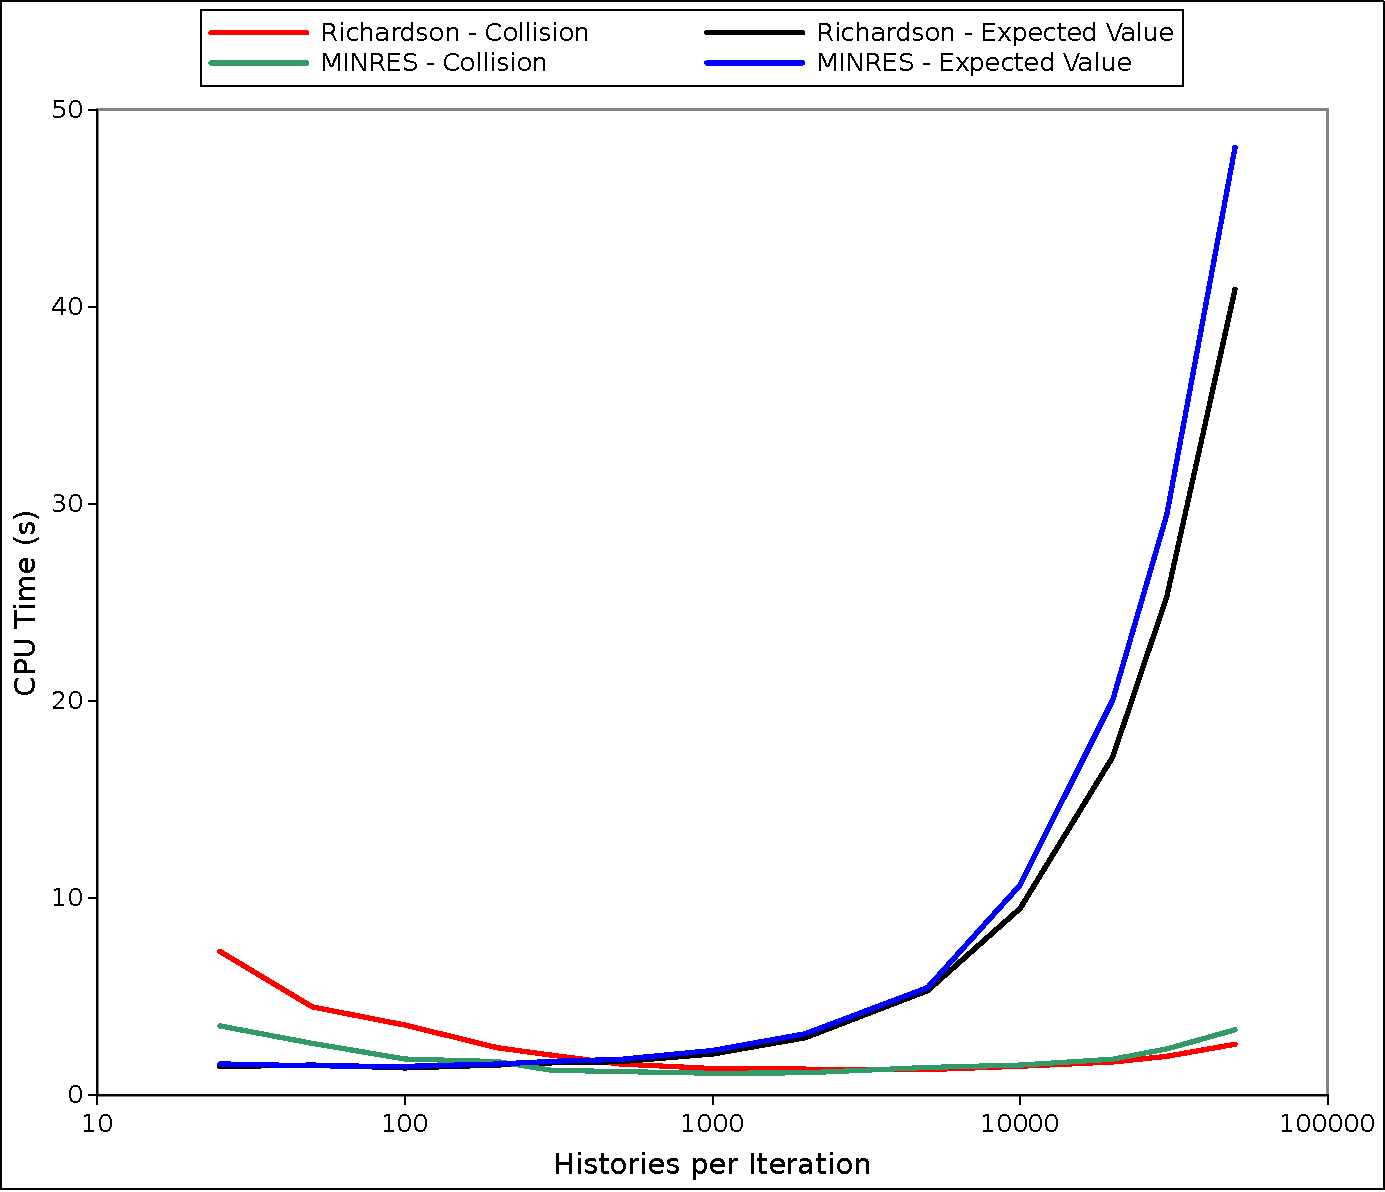
\includegraphics[width=5in]{chapters/spn_equations/estimator_time.pdf}
  \end{center}
  \caption{\textbf{Total CPU time in seconds required to converge the
      fuel assembly problem to a tolerance of \sn{1}{-8}.}
    \textit{Both the collision and expected value estimators were used
      with the adjoint Monte Carlo solver to compute the correction at
      each iteration. Each estimator was used with the Richardson and
      minimal residual fixed point iterations within an MCSA
      iteration.}}
  \label{fig:spn_estimator_time}
\end{figure}
